\documentclass[manuscript,screen,review,anonymous]{acmart}
\usepackage{xcolor}
\usepackage{mathtools}
% \documentclass[acmsmall,sigconf]{acmart}

% %% Rights management information.  This information is sent to you
% %% when you complete the rights form.  These commands have SAMPLE
% %% values in them; it is your responsibility as an author to replace
% %% the commands and values with those provided to you when you
% %% complete the rights form.
% \setcopyright{acmlicensed}
% \copyrightyear{2018}
% \acmYear{2018}
% \acmDOI{XXXXXXX.XXXXXXX}

% %% These commands are for a PROCEEDINGS abstract or paper.
% \acmConference[Conference acronym 'XX]{Make sure to enter the correct
%   conference title from your rights confirmation emai}{June 0--05,
%   2018}{Woodstock, NY}
% %%
% %%  Uncomment \acmBooktitle if the title of the proceedings is different
% %%  from ``Proceedings of ...''!
% %%
% %%\acmBooktitle{Woodstock '18: ACM Symposium on Neural Gaze Detection,
% %%  June 03--05, 2018, Woodstock, NY}
% \acmISBN{978-1-4503-XXXX-X/18/06}

\usepackage{mathtools}
\usepackage{multirow}
\usepackage{subcaption}
\usepackage{algorithm}
\usepackage{algorithmic}

\graphicspath{{images/}}
\DeclareGraphicsExtensions{.pdf}

\DeclarePairedDelimiter{\set}{\{}{\}}
\DeclarePairedDelimiter{\tuple}{(}{)}
\DeclarePairedDelimiter{\abs}{\lvert}{\rvert}
\renewcommand{\implies}{\rightarrow}
\newcommand{\db}{D}
\newcommand{\dbs}{\mathcal{D}}
\newcommand{\model}{\mathcal{M}}
\newcommand{\priv}{R}
\newcommand{\pos}{\hat{P}}
\newcommand{\posm}{\hat{P}_\mathcal{M}}
\newcommand{\tru}{T}
\newcommand{\leg}{L}
\newcommand{\sco}{\hat{S}}
\newcommand{\scom}{\hat{S}_\mathcal{M}}
\newcommand{\calib}{C}
\newcommand{\prob}[1]{\text{Pr}[#1]}
\newcommand{\mi}[2]{I(#1;#2)}
\newcommand{\entropy}[1]{H(#1)}

%%
%% end of the preamble, start of the body of the document source.
\begin{document}

%%
%% The "title" command has an optional parameter,
%% allowing the author to define a "short title" to be used in page headers.
\title{Quantitative Auditing of AI Fairness with Differentially Private Synthetic Data}

%%
%% The "author" command and its associated commands are used to define
%% the authors and their affiliations.
%% Of note is the shared affiliation of the first two authors, and the
%% "authornote" and "authornotemark" commands
%% used to denote shared contribution to the research.
\author{Chih-Cheng Rex Yuan}
\email{hello@rexyuan.com}
\affiliation{%
  \institution{Institute of Information Science, Academia Sinica}
  \city{Taipei}
  \country{Taiwan}
}

\author{Bow-Yaw Wang}
\email{bywang@iis.sinica.edu.tw}
\affiliation{%
  \institution{Institute of Information Science, Academia Sinica}
  \city{Taipei}
  \country{Taiwan}
}

%%
%% By default, the full list of authors will be used in the page
%% headers. Often, this list is too long, and will overlap
%% other information printed in the page headers. This command allows
%% the author to define a more concise list
%% of authors' names for this purpose.
% \renewcommand{\shortauthors}{Trovato et al.}

%%
%% The abstract is a short summary of the work to be presented in the
%% article.
\begin{abstract}
Ensuring fairness in AI systems is crucial, but auditing these systems often requires sensitive data, which raises security and privacy concerns. To address this, we introduce a framework that utilizes differentially private synthetic data for fairness evaluations. This approach allows auditors to assess AI systems without exposing sensitive information. Through experiments on datasets like Adult, COMPAS, and Diabetes, we compare fairness metrics of synthetic and real data. Our results ... (to be continued)
\end{abstract}

% %%
% %% The code below is generated by the tool at http://dl.acm.org/ccs.cfm.
% %% Please copy and paste the code instead of the example below.
\begin{CCSXML}
  <ccs2012>
     <concept>
         <concept_id>10002944.10011123.10011124</concept_id>
         <concept_desc>General and reference~Metrics</concept_desc>
         <concept_significance>500</concept_significance>
         </concept>
     <concept>
         <concept_id>10002978.10003029.10011703</concept_id>
         <concept_desc>Security and privacy~Usability in security and privacy</concept_desc>
         <concept_significance>500</concept_significance>
         </concept>
     <concept>
         <concept_id>10002951.10003227.10003351</concept_id>
         <concept_desc>Information systems~Data mining</concept_desc>
         <concept_significance>300</concept_significance>
         </concept>
     <concept>
         <concept_id>10010147.10010257</concept_id>
         <concept_desc>Computing methodologies~Machine learning</concept_desc>
         <concept_significance>300</concept_significance>
         </concept>
     <concept>
         <concept_id>10010147.10010178</concept_id>
         <concept_desc>Computing methodologies~Artificial intelligence</concept_desc>
         <concept_significance>300</concept_significance>
         </concept>
     <concept>
         <concept_id>10002978.10002991.10002995</concept_id>
         <concept_desc>Security and privacy~privacy-preserving protocols</concept_desc>
         <concept_significance>300</concept_significance>
         </concept>
     <concept>
         <concept_id>10002951.10003227</concept_id>
         <concept_desc>Information systems~Information systems applications</concept_desc>
         <concept_significance>300</concept_significance>
         </concept>
     <concept>
         <concept_id>10002950.10003648.10003688.10003690</concept_id>
         <concept_desc>Mathematics of computing~Contingency table analysis</concept_desc>
         <concept_significance>300</concept_significance>
         </concept>
   </ccs2012>
\end{CCSXML}

\ccsdesc[500]{General and reference~Metrics}
\ccsdesc[500]{Security and privacy~Usability in security and privacy}
\ccsdesc[300]{Information systems~Data mining}
\ccsdesc[300]{Computing methodologies~Machine learning}
\ccsdesc[300]{Computing methodologies~Artificial intelligence}
\ccsdesc[300]{Security and privacy~privacy-preserving protocols}
\ccsdesc[300]{Information systems~Information systems applications}
\ccsdesc[300]{Mathematics of computing~Contingency table analysis}

\keywords{AI, fairness, auditing, differential privacy, synthetic data}

% \received{20 February 2007}
% \received[revised]{12 March 2009}
% \received[accepted]{5 June 2009}

\maketitle

\section{Introduction}

% fairness

Fairness in machine learning has become an important topic as AI systems become widely used. Biased AI systems could result in amplified unfairness. Ensuring fairness in AI systems is crucial to prevent these biases from being exacerbated by AI systems. One approach is to audit the fairness of existing AI systems. Quantitative fairness auditing is a process of evaluating the fairness of AI systems with a range of fairness metrics. Many metrics have been proposed to help evaluate the fairness of AI systems.

Auditing can evaluate the fairness of AI systems, sometimes revealing cases of unfairness in them. For example, investigative journalists at ProPublica found that the COMPAS system, which is used to predict recidivism in the criminal justice system in the United States, is biased against certain demographic groups. This highlights the need for fairness auditing conducted by third parties.

% data privacy

To conduct audits, auditors may rely on access to real datasets containing sensitive information, raising significant security and privacy concerns. This reliance invites data security attacks on auditors, making them targets of unauthorized access. Analysis on real data runs the risk of data inference attacks, where confidential information may be deduced from seemingly harmless or aggregated data. Various technologies have been developed to mitigate these risks, such as differential privacy, where the idea is that whether or not any individual is in a dataset has a limited impact.

To mitigate these risks, the use of synthetic data has been proposed. Synthetic data are fake data that is artificially generated from real data. The principle of this technology is to preserve some statistical properties of the real data while protecting the privacy of the individuals in the real data. Among the generation techniques, differentially private synthetic data offers a way to investigate the data properties under differential privacy guarantees.

% differentially private synthetic data for fairness auditing

We propose a novel auditing framework that leverages differentially private synthetic data to evaluate the fairness of AI systems. Our framework lets the auditors assess the fairness of AI systems without exposing sensitive information. Differentially private synthetic data is a technique that generates synthetic data from real data that preserves some statistical properties of the real data while ensuring differential privacy. This technology enables auditing without exposing sensitive information. However, synthetic data also introduces new challenges. Whether or not it accurately preserves the fairness properties of the real data is a critical question.

% contribution

Our work examines the capabilities of existing differentially private synthetic data generation technologies in preserving fairness properties. Through empirical experiments on multiple real datasets, we aim to determine the effectiveness of differentially private synthetic data in this respect.

\section{Related Work}

% fairness

Fairness in machine learning has become a crucial area of research\cite{barocas2023fairness}. Various fairness measures have been proposed to quantify\cite{yeh2024analyzing} the fairness of AI models\cite{pessach2022review,corbett2017algorithmic,vzliobaite2017measuring,hardt2016equality,corbett2017algorithmic,berk2021fairness,chouldechova2017fair,kleinberg2016inherent}. We consider these fairness measures in this work.

Auditing of AI models is an important step in ensuring that these models are fair\cite{ferrara2023fairness}. Different tools have been developed to check the fairness of AI models\cite{saleiro2018aequitas,bellamy2019ai,bird2020fairlearn}. We use a tool produced from our previous work\cite{yuan2024ensuring}.

% differential privacy

Differential privacy has risen to become the standard of privacy protection in many data analyses\cite{jiang2021applications}. It offers a formal framework for quantifying privacy guarantees when releasing information derived from sensitive data\cite{dwork2006calibrating,dwork2014algorithmic}. We use differential privacy in this work to protect the privacy of individuals in the data in our auditing framework.

Different flavors of differential privacy have been proposed over the years\cite{desfontaines2019sok}, such as Gaussian differential privacy\cite{dong2022gaussian}, Pufferfish differential privacy\cite{kifer2012rigorous}, Bayesian differential privacy\cite{triastcyn2020bayesian}, and R\'enyi differential privacy\cite{mironov2017renyi}. We consider R\'enyi differential privacy specifically in this work.

% synthetic data

The generation of synthetic data\cite{raghunathan2021synthetic,lu2023machine} under differential privacy constraints allows for data sharing without compromising privacy\cite{tao2021benchmarking}. There have been several techniques developed for differentially private synthetic data generation\cite{rosenblatt2020differentially,fan2020relational,bowen2019comparative,bowen2020comparative,arnold2020really,xu2019modeling} in recent years. We use the technique that won the 2018 NIST differential privacy Synthetic Data Challenge competition\cite{mckenna2021winning}.

There have also been some works that aim to alter the properties of synthetic data, such as introducing bias to them\cite{jiang2024synthetic,baumann2023bias}. In this work, we aim to preserve the properties of the original data. Thus, we do not consider these works.

While helpful, there are some technical limitations\cite{stadler2022synthetic,cheng2021can,ganev2022robin,wyllie2024fairness} and ethical concerns\cite{whitney2024real} with the use of synthetic data. Synthetic data may not always preserve properties of real data. This may cause inaccuracies in downstream tasks such as fairness evaluation. Our work examines these limitations.

\section{Preliminaries}
\label{sec:prelim}

Let $\prod_i x_i$ denote the Cartesian product of $x_i$s.

An \emph{attribute} is a symbol $A$.
The set of all attributes is $\mathcal{A}$.
An \emph{attribute value} is a symbol $a$.
The set of all attribute values is $\Omega$.
An \emph{attribute value space} is a function $\sigma : \mathcal{A} \implies 2^{\Omega}$
specifying the set of valid values that attributes can take on.
A \emph{row} with respect to $\sigma$
is a function $r : \mathcal{A} \implies \Omega$
where $r(A) \in \sigma(A)$.
The set of all rows is $\mathcal{R}$.
A \emph{database} is a tuple $\db =
\tuple{
    \mathcal{A}_{\db},
    \Omega_{\db},
    \sigma_{\db},
    \mathcal{R}_{\db}
}$
where
$\mathcal{A}_{\db} \subseteq \mathcal{A}$
is the set of attributes in $\db$,
$\Omega_{\db} \subseteq \Omega$
is the set of attribute values in $\db$,
$\sigma_{\db} : \mathcal{A}_{\db} \implies 2^{\Omega_{\db}}$
is the function specifying the valid values that each attribute can take on in $\db$,
and $\mathcal{R}_{\db} \subseteq \mathcal{R}$
is the set of rows with respect to $\sigma_{\db}$ in $\db$
with $r_\db : \mathcal{A}_\db \implies \Omega_\db$
for all $r_\db \in \mathcal{R}_\db$
and $r_\db(A) \in \sigma_\db(A)$
for all $A \in \mathcal{A}_\db$.
The set of all databases is $\dbs$.

Let $X \in \mathcal{X},Y \in \mathcal{Y}$ be discrete random variables. Their \emph{mutual information} $\mi{X}{Y}$ is
\[
\mi{X}{Y} = \sum_{x \in \mathcal{X}} \sum_{y \in \mathcal{Y}} P_{(X,Y)}(x,y) \text{log} \frac{P_{(X,Y)}(x,y)}{P_X(x)P_Y(y)}
\]
where $P_{(X,Y)}$ is the joint probability distribution of $X,Y$ and $P_X,P_Y$ are the marginal probability distributions of $X,Y$ respectively.
It quantifies the level of dependency between $X$ and $Y$.
% By definition\cite{427884}, the joint entropy is greater than or equal to the marginal entropies $\entropy{X,Y} \geq \text{max}(\entropy{X},\entropy{Y})$. Hence, we have an upper bound of mutual information $\mi{X}{Y} \leq \text{min}(\entropy{X}, \entropy{Y})$.

Let $\set{X_i}$ be a set of discrete random variables indexed by a graph $G = (V,E)$, where $V$ represents the random variables $X_i$s and $E$ represents dependencies between these random variables. A \emph{Markov random field} is a probability distribution over $X_i$s, such that each random variable $X_i$, given its neighborhood in $G$, is conditionally independent of all other variables. Since edges represent dependencies, cliques in a Markov random field represent groups of variables that are all mutually dependent. As a machine learning model, there has been much development in the estimation and inference of Markov random fields\cite{koller2009probabilistic,murphy2023probabilistic}.

\subsection{Fairness Measures}

For fairness measures\cite{yuan2024ensuring,pessach2022review}, let $Y$ denote the ground truth of an outcome, let $\hat{Y}$ denote the predicated result of an outcome, let $S$ denote the protected attribute, and let $\epsilon$ denote some threshold. $Y, \hat{Y}, S$ are binary.

Fairness measures can be broadly categorized into independence, separation, and sufficiency, which are defined by conditional independence in Table~\ref{tab:categories}. $X \bot Y | Z$ denotes the conditional independence between $X$ and $Y$ conditioning on $Z$.

\begin{table}[h]
\caption{Fairness categories.}
\label{tab:categories}
\begin{tabular}{cc}
\toprule
\textbf{Category} & \textbf{Definition} \\
\midrule
Independence & $S \bot \hat{Y}$ \\
Separation & $S \bot \hat{Y} | Y$ \\
Sufficiency & $S \bot Y | \hat{Y}$ \\
\bottomrule
\end{tabular}
\end{table}

These categories can be expanded into forms of probability. For example, the definition of separation is expanded to
\begin{align*}
P[\hat{Y} = 1 | S = 1, Y = 1] & = P[\hat{Y} = 1 | S \neq 1, Y = 1] \\
P[\hat{Y} = 1 | S = 1, Y = 0] & = P[\hat{Y} = 1 | S \neq 1, Y = 0]
\end{align*}
The definition can be relaxed. Its relaxation, for some parameter $\epsilon$, is
\begin{align*}
\abs{P[\hat{Y} = 1 | S = 1, Y = 1] - P[\hat{Y} = 1 | S \neq 1, Y = 1]} & \leq \epsilon \\
\abs{P[\hat{Y} = 1 | S = 1, Y = 0] - P[\hat{Y} = 1 | S \neq 1, Y = 0]} & \leq \epsilon
\end{align*}
which is also the definition of a fairness measure called equalized odds.

We consider in this work various fairness measures listed in Table~\ref{tab:measures}.

\begin{table*}[h]
\caption{Fairness measures.}
\label{tab:measures}
\begin{tabular}{lll}
\toprule
\textbf{Category} & \textbf{Fairness Measure} & \textbf{Definition} \\
\midrule
\multirow{1}{*}{Independence}
% & Disparate Impact & $\frac{P[\hat{Y} = 1 | S \neq 1]}{P[\hat{Y} = 1 | S = 1]} \geq 1 - \epsilon$ \\
& Demographic Parity & $\abs{P[\hat{Y} = 1 | S = 1] - P[\hat{Y} = 1 | S \neq 1]} \leq \epsilon$ \\
% & Conditional Statistical Parity & $\abs{P[\hat{Y} = 1 | S = 1, L = l] - P[\hat{Y} = 1 | S \neq 1, L = l]} \leq \epsilon$ \\
% & Mean difference & $\abs{E[\hat{Y}|S = 1] - E[\hat{Y}|S \neq 1]} \leq \epsilon$ \\
\multirow{2}{*}{Separation}
& \multirow{1}{*}{Equalized Odds (False Positive)} & $\abs{P[\hat{Y} = 1 | S = 1, Y = 0] - P[\hat{Y} = 1 | S \neq 1, Y = 0]} \leq \epsilon$ \\
& \multirow{1}{*}{Equalized Odds (True Positive)} & $\abs{P[\hat{Y} = 1 | S = 1, Y = 1] - P[\hat{Y} = 1 | S \neq 1, Y = 1]} \leq \epsilon$ \\
% & Equal Opportunity & $\abs{P[\hat{Y} = 1 | S = 1, Y = 1] - P[\hat{Y} = 1 | S \neq 1, Y = 1]} \leq \epsilon$ \\
% & Predictive Equality & $\abs{P[\hat{Y} = 1 | S = 1, Y = 0] - P[\hat{Y} = 1 | S \neq 1, Y = 0]} \leq \epsilon$ \\
\multirow{2}{*}{Sufficiency}
& \multirow{1}{*}{Conditional Use Accuracy Equality (True Positive)} & $\abs{P[Y = 1 | S = 1, \hat{Y} = 1] - P[Y = 1 | S \neq 1, \hat{Y} = 1]} \leq \epsilon$ \\
& \multirow{1}{*}{Conditional Use Accuracy Equality (True Negative)} & $\abs{P[Y = 0 | S = 1, \hat{Y} = 0] - P[Y = 0 | S \neq 1, \hat{Y} = 0]} \leq \epsilon$ \\
% & Predictive Parity & $\abs{P[Y = 1 | S = 1, \hat{Y} = 1] - P[Y = 1 | S \neq 1, \hat{Y} = 1]} \leq \epsilon$ \\
% & Equal Calibration & $\abs{P[Y = 1 | S = 1, \hat{V} = v] - P[Y = 1 | S \neq 1, \hat{V} = v]} \leq \epsilon$ \\
\multirow{1}{*}{N/A}
& Overall Accuracy Equality & $\abs{P[Y = \hat{Y} | S = 1] - P[Y = \hat{Y} | S \neq 1]} \leq \epsilon$ \\
% & Positive Balance & $\abs{E[\hat{V} | Y = 1, S = 1] - E[\hat{V} | Y = 1, S \neq 1]} \leq \epsilon$ \\
% & Negative Balance & $\abs{E[\hat{V} | Y = 0, S = 1] - E[\hat{V} | Y = 0, S \neq 1]} \leq \epsilon$ \\
\bottomrule
\end{tabular}
\end{table*}

\subsection{R\'enyi differential privacy}

% \begin{definition}[differential privacy (DP) \cite{dwork2006calibrating,dwork2014algorithmic,mckenna2021winning}]\label{def:rdp}
% A randomized mechanism $M$ satisfies $(\epsilon,\delta)$-DP if, for all databases $\db_1,\db_2$ that differ in exactly one row and for all subsets $S$ of $R$, we have
% \[
% \prob{M(\db_1) \in S} \leq e^\epsilon \prob{M(\db_2) \in S} + \delta
% \]
% \end{definition}

A \emph{randomized mechanism} is a randomized algorithm $M : \dbs \implies \mathbb{R}^p$ that takes a database and, after introducing noise, outputs some results.

Let $\db_1,\db_2$ be two databases. They are \emph{neighbors}, denoted $\db_1 \sim \db_2$, if $\abs{\mathcal{R}_{\db_1} \Delta \mathcal{R}_{\db_2}} = 1$ where $\Delta$ denotes symmetric difference; that is, one database contains an extra row than the other. In other words, they differ in exactly one row.

\begin{definition}[Gaussian Mechanism\cite{dwork2014algorithmic}]\label{def:gm}
Let $f : \dbs \implies \mathbb{R}^p$ be a function. The Gaussian Mechanism $M$ adds independent and identically distributed Gaussian noise with mean $0$ and standard deviation $\sigma$ to each component of the $p$-dimensional vector output of $f(\db)$
\[
M(\db) = f(\db) + \mathcal{N}(0_p, \sigma^2 \mathbb{I}_p)
\]
where $\mathcal{N}$ is a multivariate normal distribution with mean vector $0_p$ and covariance matrix $\sigma^2 \mathbb{I}_p$ where $\mathbb{I}_p$ is the identity matrix.
\end{definition}

\begin{definition}[R\'enyi Differential Privacy (RDP)]\label{def:rdp}
Let $P_{\mathbf{X}}$ denote the probability distribution associated with the random vector $\mathbf{X}$. A randomized mechanism $M$ satisfies $(\alpha,\gamma)$-RDP for $\alpha \geq 1$ and $\gamma \geq 1$ if, for all databases $\db_1 \sim \db_2$, we have
\[
D_\alpha(P_{M(\db_1)} \Vert P_{M(\db_2)}) \leq \gamma
\]
where $D_\alpha(P_1 \Vert P_2)$ is the R\'enyi divergence\cite{van2014renyi,van2010renyi,li2016renyi} of order $\alpha$ between probability distributions $P_1,P_2$ over $x$
\[
D_\alpha(P_1 \Vert P_2) := \frac{1}{\alpha - 1} \text{log} \int {P_1(x)}^\alpha {P_2(x)}^{1-\alpha} \text{d}x
\]
\end{definition}

\begin{theorem}[RDP of the Gaussian Mechanism\cite{feldman2018privacy,mironov2017renyi}]
The Gaussian Mechanism satisfies $(\alpha, \alpha \frac{\Delta^2_f}{2 \sigma^2})$-RDP, where $\Delta_f$ denotes the sensitivity\cite{dwork2014algorithmic} of $f$, which is defined as the maximum $L^2$-norm difference in the output of $f$
\[
\Delta_f := \text{max}_{\db_1 \sim \db_2} \Vert f(\db_1) - f(\db_2) \Vert_2
\]
\end{theorem}

\subsection{Differentially Private Synthetic Data}

Let $C \subseteq \mathcal{A}$ be a subset of attributes. Let $\Omega_C = \prod_{i \in C} \Omega_i$. Let $x$ be a row and $x_C$ denote the restriction of $x$ to $C$. A \emph{marginal}\cite{barak2007privacy,mckenna2021winning} of $C$ on database $\db$ is a function $\mu_{\db} : \Omega_C \implies \mathbb{N}_0$ such that $\mu_{\db}(t) = \Sigma_{x \in \mathcal{\db}} \delta_{t,{x_C}}$ where $\delta$ is the Kronecker function; that is, it is a lookup table of the counts of each possible combination of attribute values. We call marginals of $|C| = n$ attributes $n$-way marginals.

The task of differentially private synthetic data\cite{Ullman2022,McKenna2022,NIST_Differentially_Private_Synthetic_Data,YouTube_Differentially_Private_Synthetic_Data} is, given a database $\db$, adding some noise to marginals of $\db$ such that it satisfies some differential privacy guarantees and outputting another database $\db'$, such that the $L^1$-norm errors between marginals of $\db$ and $\db'$ is small; that is, their marginals $\mu_{\db},\mu_{\db'}$ are similar.

For example, suppose we have a database with attributes sex and race. The 2-way marginals of the original database and the synthetic database are shown in Table~\ref{tab:marginal-example}. The marginals of the synthetic data is supposed to be similar to that of the original database.

\begin{table}[h]
\caption{Example marginals.}
\label{tab:marginal-example}
\centering
\begin{subtable}[t]{0.45\linewidth}
\centering
\caption{Marginal of original data.}
\begin{tabular}{lr}
\toprule
Attributes & Count \\
\midrule
Male,White & 24 \\
Female,White & 33 \\
Male,Black & 13 \\
Female,Black & 47 \\
\bottomrule
\end{tabular}
\end{subtable}
\begin{subtable}[t]{0.45\linewidth}
\centering
\caption{Marginal of synthetic data.}
\begin{tabular}{lr}
\toprule
Attributes & Count \\
\midrule
Male,White & 22 \\
Female,White & 35 \\
Male,Black & 10 \\
Female,Black & 46 \\
\bottomrule
\end{tabular}
\end{subtable}
\end{table}

\section{Motivation}

AI systems are widely used in various aspects in our society. However, these systems may be biased against certain demographic groups. For example, COMPAS, the AI system used in American criminal justice system to predict recidivism, has been found to be biased by ProPublica, a third party media.

To ensure the fairness of AIs, third-party audits such as this is crucial. Auditing can reveal instances of unfairness in AI systems, allowing for corrective actions to be taken. We hence advocate for a framework that centers around third-party audits.

Our auditing framework is tripartite. It consists of three parties: the data provider, the model maker, and the third-party auditor. The COMPAS investigation could fit in with this framework.

The data provider is responsible for supplying the raw datasets which should originate from trustworthy sources, such as government agencies like a census bureau. In the COMPAS example, the data provider is the government agencies that provide criminal justice data, such as the Broward County Sheriff's Office in Florida.

The model maker develops AI models. These are AI companies or research labs specialized in training and optimizing AI models. The model maker in the COMPAS example is Northpointe, Inc., the company that developed the COMPAS system.

The third-party auditor acts as an evaluator, using our tool to audit the AI models for fairness issues by combining both the datasets and the models. These may be investigative journalists or regulatory bodies. ProPublica is the third-party auditor in the COMPAS example, using quantitative methods to evaluate the fairness of the COMPAS system using Florida's data.

\begin{figure}[h]
  \centering
  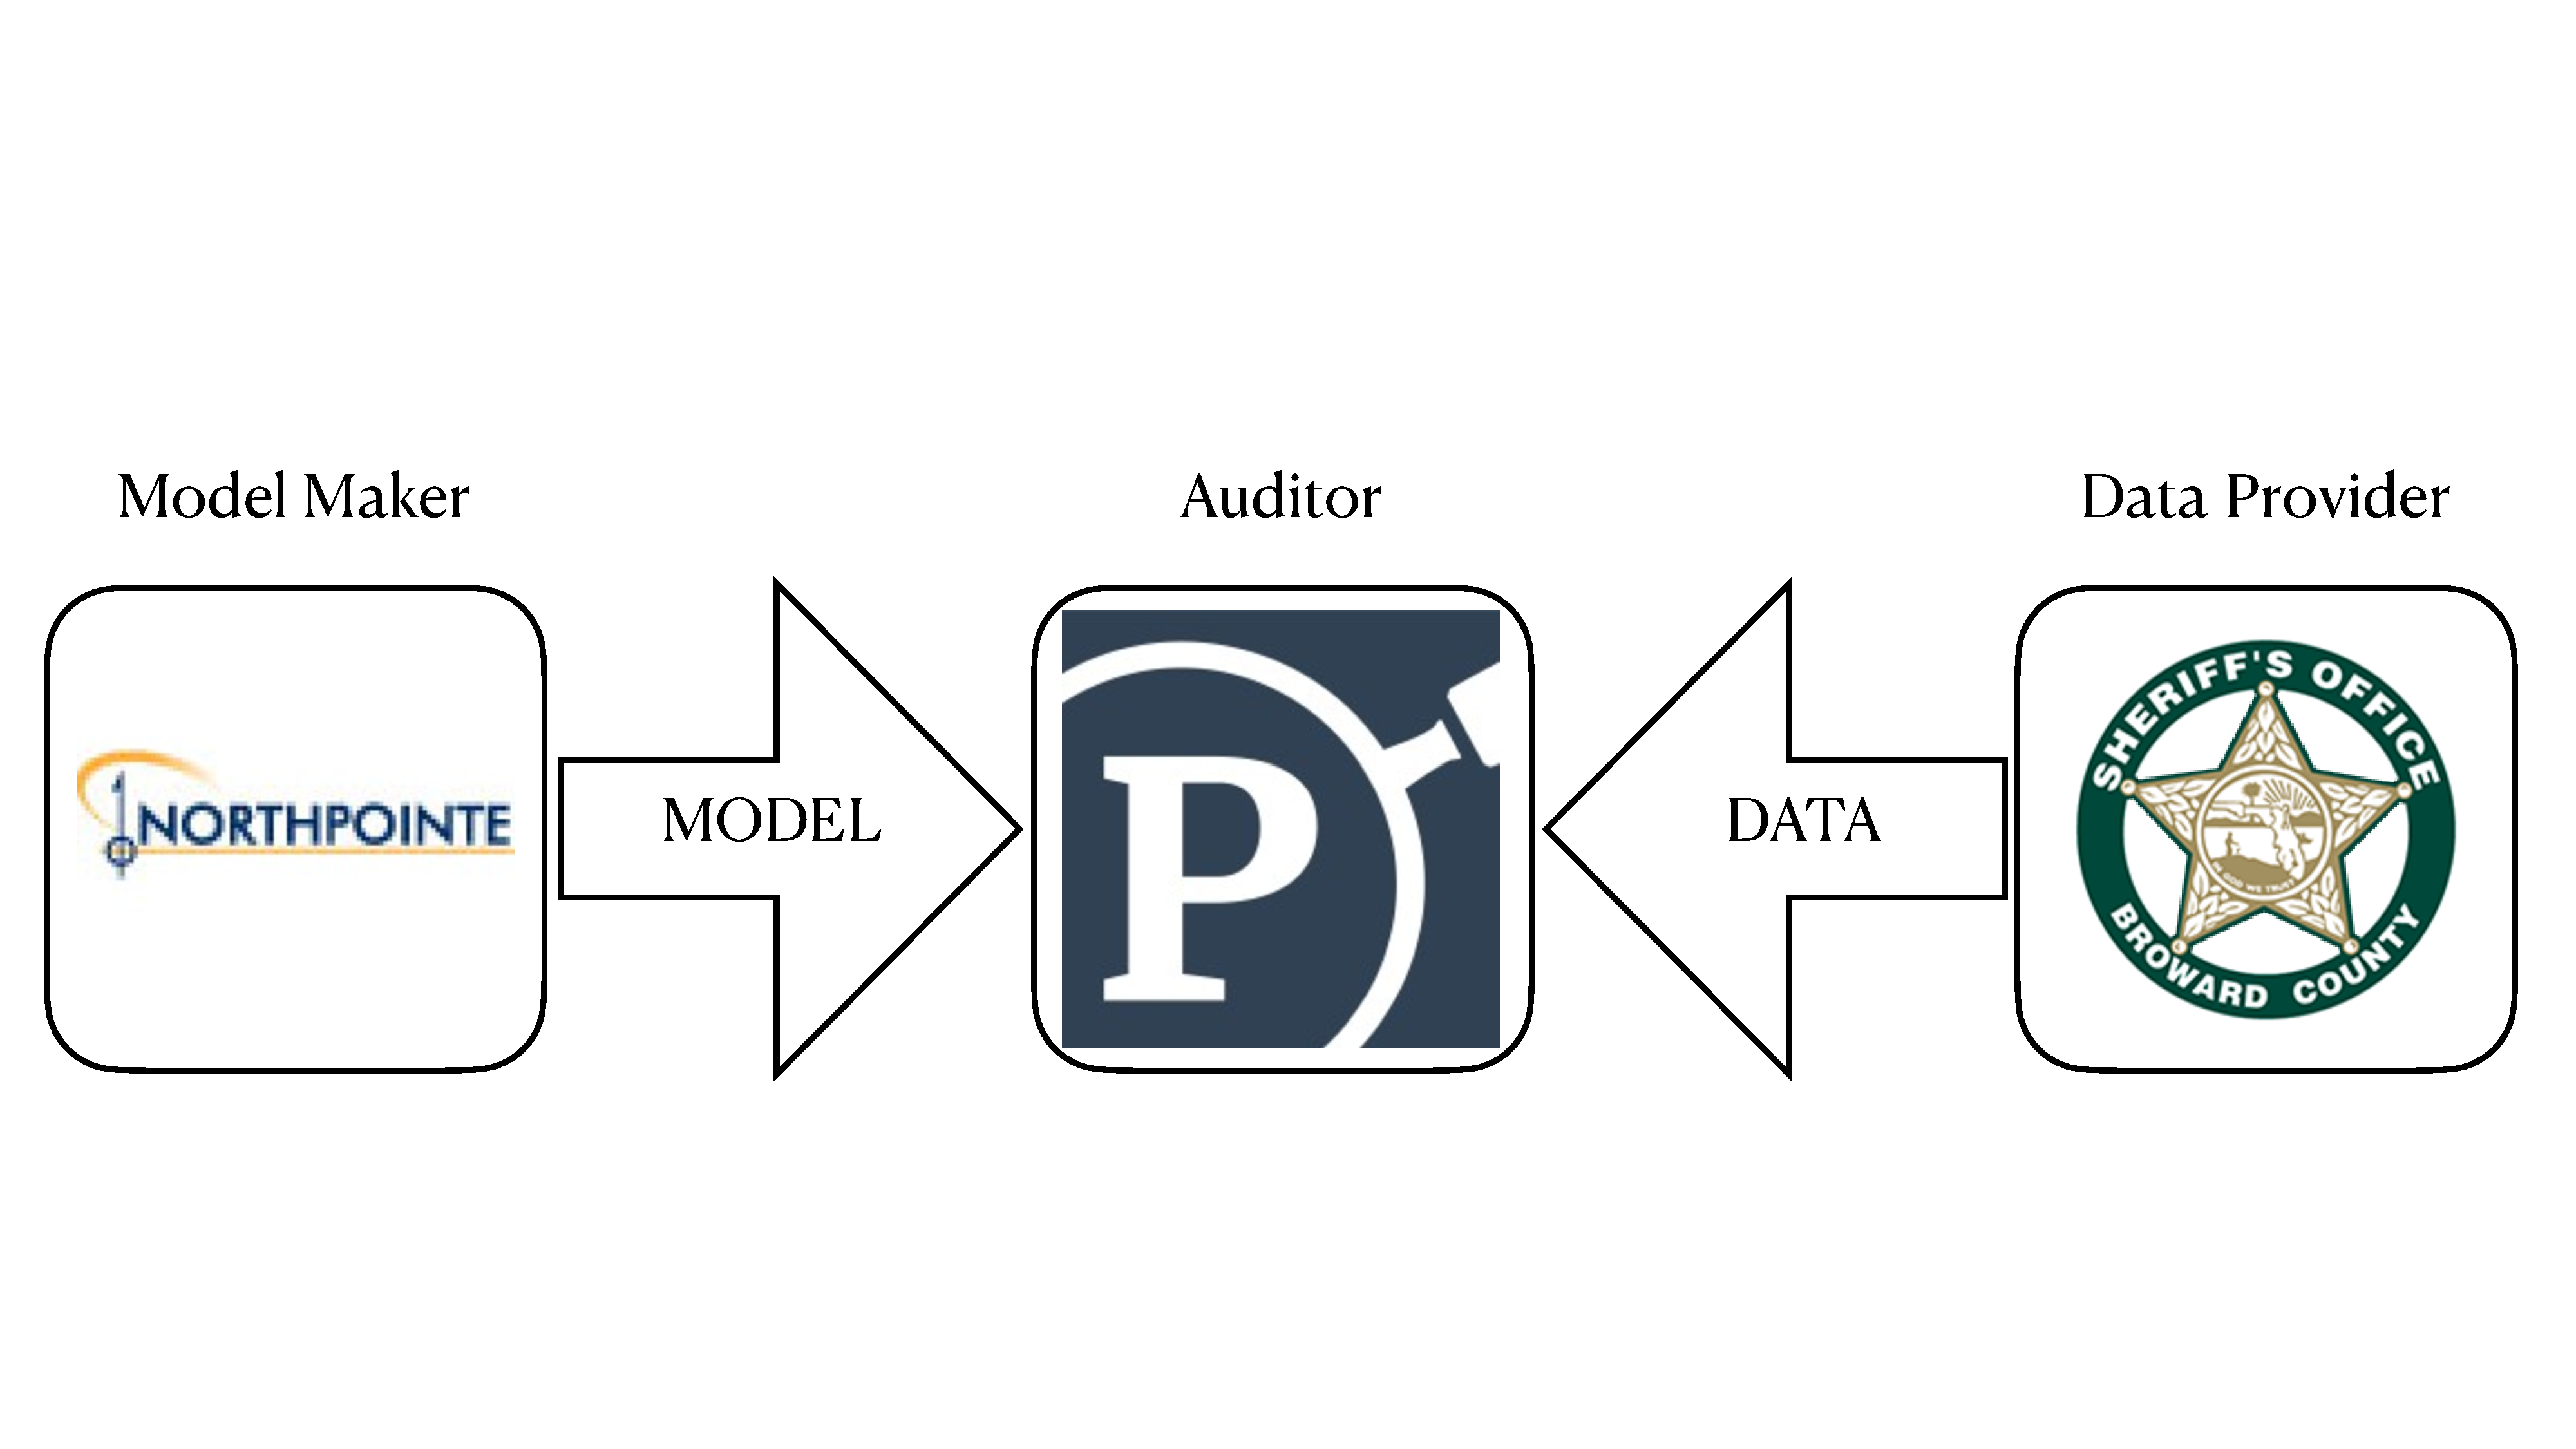
\includegraphics[width=\linewidth]{compas}
  \caption{Roles of each party in the COMPAS example.}
  \label{fig:compas}
  \Description{Roles of each party in the COMPAS example.}
\end{figure}

In the framework of our previous work\cite{yuan2024ensuring}, after obtaining real data from the data provider, the 3rd party auditor holds onto the real data for performing fairness audits, and it supposedly retains it indefinitely for the possibility of any future audits. However, this practice raises both security and privacy concerns.

For security, it creates a point of vulnerability to unauthorized access, and the auditor is now a target of data security attacks. The auditor may not have the necessary resources to defend against these threats. A breach at the auditor's end could result in compromises of individuals' sensitive information. In the COMPAS example, had the data not been public already, ProPublica may be targeted by hackers to access the sensitive criminal justice data.

As for privacy, on the other hand, it introduces risks of information leakage. Releasing analyses of real data may inadvertently reveal sensitive information through data inference attacks. Attackers can exploit data patterns in outputs or combine outputs with external data to infer sensitive information. In the COMPAS example, had the data not been public already, their analyses may inadvertently reveal the identities of individuals in the criminal justice system.

Thus, we introduce a new framework where the auditor generates synthetic data based on real data upon retrieval of the real data, and then holds onto the synthetic data and discards the real data, preventing all further security and privacy violations. The third-party still retains the ability to audit all incoming future models as needed.

\section{Methodology}
\label{sec:method}

We employed the tools of the winner of the 2018 NIST differential privacy Synthetic Data Challenge competition\cite{NIST2018} by \cite{nist_ryan_2018,McKenna_private-PGM_2021,mckenna2021winning,mckenna2019graphical} and the fairness checker tool from our previous research\cite{yuan2024ensuring}.

This research is conducted in Python Jupyter notebooks and is publicly available.

We shall illustrate the workflow of our methodology with an example of the COMPAS dataset, which contains attributes such as sex and race with the prediction target attribute being recidivism.

\subsection{Data Synthesis}

The synthesis framework is three-fold, namely, select-measure-generate\cite{McKenna2022,YouTube_Differentially_Private_Synthetic_Data}. We first select the important marginals to preserve, measure them by adding differential privacy noise, and then generate synthetic data.

Underneath the hood, the tool employs a Markov random field. The select step corresponds to marking cliques in a Markov random field, and the generate step corresponds to sampling from the fitted Markov random field.

By default, all $1$-way marginals are selected to preserve the quantity of each attribute element. We can further preserve correlations by adding $n$-way marginals. For example, if we want to preserve the relationship between sex and race, we may add the clique (sex,race).

In a perfect world where all correlation information is to be preserved, we may wish to make a complete graph. However, this is intractable as the complexity of the problem would skyrocket. Furthermore, algorithms for Markov random field favor graphs with specific shapes, such as trees.

To circumvent this complexity explosion, instead, \cite{mckenna2021winning} devised a technique where the mutual information of all the database attribute pairs is calculated, and then a maximum spanning tree is identified with edge weights being the mutual information to obtain a skeleton tree-shaped Markov random field. The marginals are then selected based on the edges of this tree.

For the competition, \cite{mckenna2021winning} further manually added certain cliques based on his investigation of the competition dataset. For example, they manually added the clique (sex,city,income). In addition, they would add some edges based on some sophisticated heuristics tailored to that particular dataset. We do not consider these additional heuristics for the generality of our approach. Meanwhile, his other apporach where the auditor does access the real dataset does not fit our framework.

While synthetic data generation methods often leverage domain knowledge to improve accuracy, we chose to employ a vanilla approach with only the maximum spanning tree method without incorporating additional heuristics. This decision was made due to two main factors: first, the need for more specific domain knowledge about the dataset makes it difficult to identify meaningful dependencies; second, prediction targets may differ from dataset to dataset, which means that tailored heuristics could not be effectively generalized. By avoiding dataset-specific adjustments, our method remains general and applicable to a wide range of datasets, in addition to being more computatioanlly efficient.

% We hence developed an alternative heuristic for the general-purpose workflow. As mentioned in Section~\ref{sec:prelim}, the mutual information of two random variables is bounded by the pair's respective Shannon entropy. Using this property, we add additional edges with weights exceeding a fraction of the minimum of these upper bounds. As a rule of thumb, we have found setting the fraction to be $0.1$ to be effective.

For the measure step, we followed the examples provided in the tool's repository. Gaussian noises are added to the selected marginals. Half of the privacy budget $\epsilon = 1$ is spent on all 1-way marginals and the other half on the selected cliques. These marginals are then fed to the tool to fit the Markov random field. By \cite{mckenna2021winning}, this procedure satisfies $(\alpha,\frac{\alpha}{2 \sigma^2})$-RDP for all $\alpha \geq 1$.

In the COMPAS example, we may select the marginal (sex,race). This marginal is then perturbed by Gaussian noise, as shown in Table~\ref{tab:marginal-perturbed}.

\begin{table}[h]
\caption{Example marginals.}
\label{tab:marginal-perturbed}
\centering
\begin{subtable}[t]{0.45\linewidth}
\centering
\caption{Original marginal.}
\begin{tabular}{lr}
\toprule
Attributes & Count \\
\midrule
Female,African-American & 1537 \\
Female,Asian & 8 \\
Female,Caucasian & 1465 \\
Female,Hispanic & 215 \\
Female,Native American & 15 \\
Female,Other & 143 \\
Male,African-American & 8254 \\
Male,Asian & 63 \\
Male,Caucasian & 4621 \\
Male,Hispanic & 1236 \\
Male,Native American & 42 \\
Male,Other & 717 \\
\bottomrule
\end{tabular}
\end{subtable}
\begin{subtable}[t]{0.45\linewidth}
\centering
\caption{Perturbed marginal.}
\begin{tabular}{lr}
\toprule
Attributes & Count \\
\midrule
Female,African-American & 1545.7885 \\
Female,Asian & 4.3236 \\
Female,Caucasian & 1444.7303 \\
Female,Hispanic & 208.2250 \\
Female,Native American & 26.7479 \\
Female,Other & 150.8175 \\
Male,African-American & 8296.6274 \\
Male,Asian & 92.1107 \\
Male,Caucasian & 4643.0108 \\
Male,Hispanic & 1274.0831 \\
Male,Native American & 28.9542 \\
Male,Other & 710.3473 \\
\bottomrule
\end{tabular}
\end{subtable}
\end{table}

\subsection{Fairness Checking}

After synthesizing the dataset, we used the fairness checker from \cite{yuan2024ensuring} to compute the fairness measures of any incoming AI model.

The fairness checker is an open-sourced public domain Python package that computes various fairness measures, such as those mentioned in Table~\ref{tab:measures}.

The checker is designed to be user-friendly and agnostic to the underlying AI model. It is also designed to be easily extensible to accommodate new fairness measures.

The checker simply iterates through the given database $\db$ and computes the results based on some given predicates on the rows $r_i$s, and finally outputs the fairness measure values.

Protected groups $S$, predicted outcomes $\hat{Y}$, and ground truths $Y$ are all formulated as these predicates. These are straightforward logical boolean expressions. Specifically, they are given as Python functions that output boolean values.

The interpretation of the resulting fairness measure values is dependent on the third-party auditors. The auditors may have different thresholds $\epsilon$ for different fairness measures or different AI models.

In the COMPAS example, the sensitive attribute is sex and the protected group is female, the protected group predicate would be $S := r(sex) = Female$; prediction is if a person will re-offend $\hat{Y} := \mathcal{M}_{recid}(r)$ where $\mathcal{M}$ is the model's prediction of row $r$; ground truth is whether a person does re-offend $Y := r(recid)$. These can be easily implemented in Python as a comparison function.

\section{Experiments}

To test the viability of our method, we compare the metrics computed from the synthetic dataset against those of the original dataset. We used various datasets with fairness concerns mentioned in \cite{pessach2022review}.

We looked at several publicly available datasets, such as Adult\cite{adult_2,Kaggle_Adult_Census_Income}, COMPAS\cite{larson2016propublica,Kaggle_COMPAS_Dataset}, and Diabetes\cite{diabetes_34,Kaggle_Diabetes_Prediction}. These datasets are known to have fairness issues\cite{pessach2022review}.

The fairness checker evaluates datasets based on multiple fairness metrics, such as demographic parity and equalized odds. By comparing these measures between the synthetic and original datasets, we aim to ensure that the synthetic data preserves the fairness properties of the original data. The comparison process is three-fold. It goes as follows.

The dataset is first processed so it can be fed into the synthetic data generator. Some marginals are selected according to their mutual information, as described in the Section~\ref{sec:method}, and the synthetic data generator model is fitted to the original data according to the selected marginals. Then the generator is run 100 times to obtain 100 sets of synthetic data.

Next, several AI models are extracted from various real-life authors from Kaggle. They are finetuned to perform well on the original dataset. For one, a random forest model is finetuned by searching hyperparameters settings\cite{Ipbyrne2023}. Another random forest model is finetuned with over-sampling methods\cite{Jawat2024}. Also, a logistic regression model is finetuned by performing principal component analysis\cite{Prashant1112023}.

The AI models and both the original dataset and synthetic datasets are then fed to the fairness checker. Sensitive attributes are identified based on manual examination with common sense or by referring to \cite{pessach2022review}. Then, applicable fairness measures are computed using the checker for both the original and the synthetic.

% \begin{figure}[h]
%   \centering
%   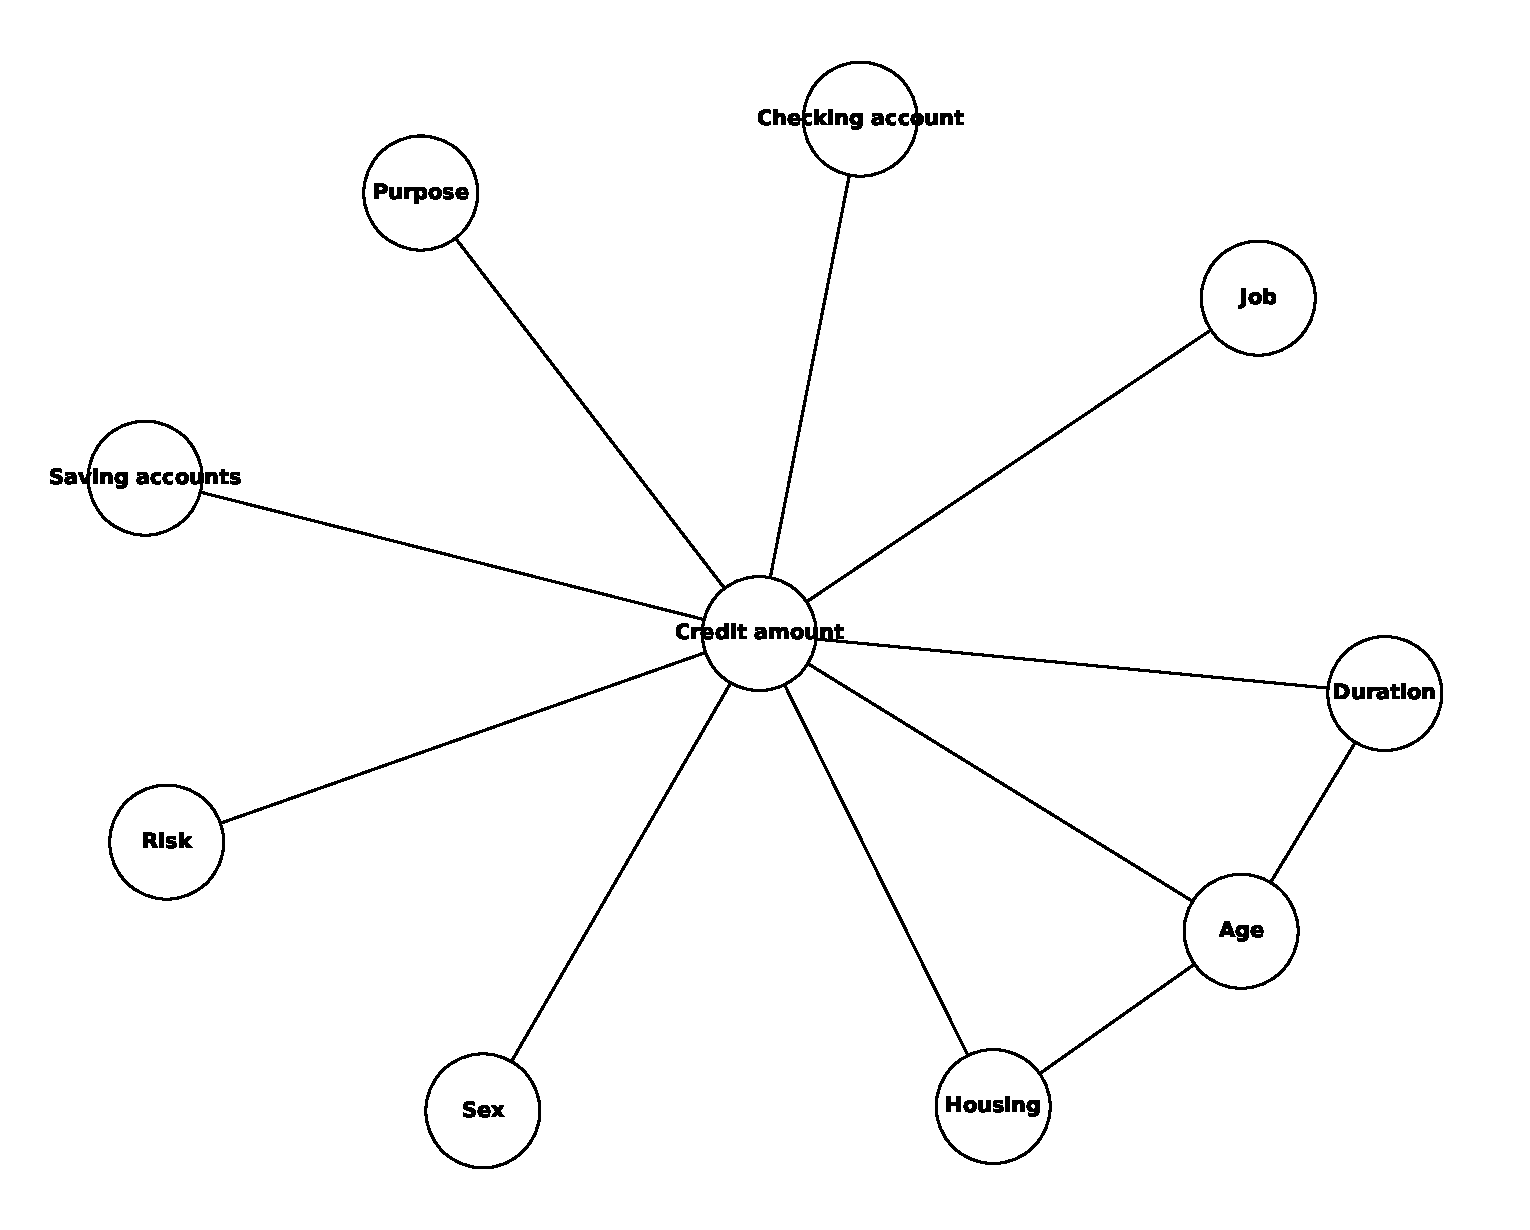
\includegraphics[width=\linewidth]{adult_mst}
%   \caption{Markov random field for marginals of the adult dataset.}
%   \label{fig:adult_mst}
%   \Description{Markov random field for marginals of the adult dataset.}
% \end{figure}

% \begin{figure}[h]
%   \centering
%   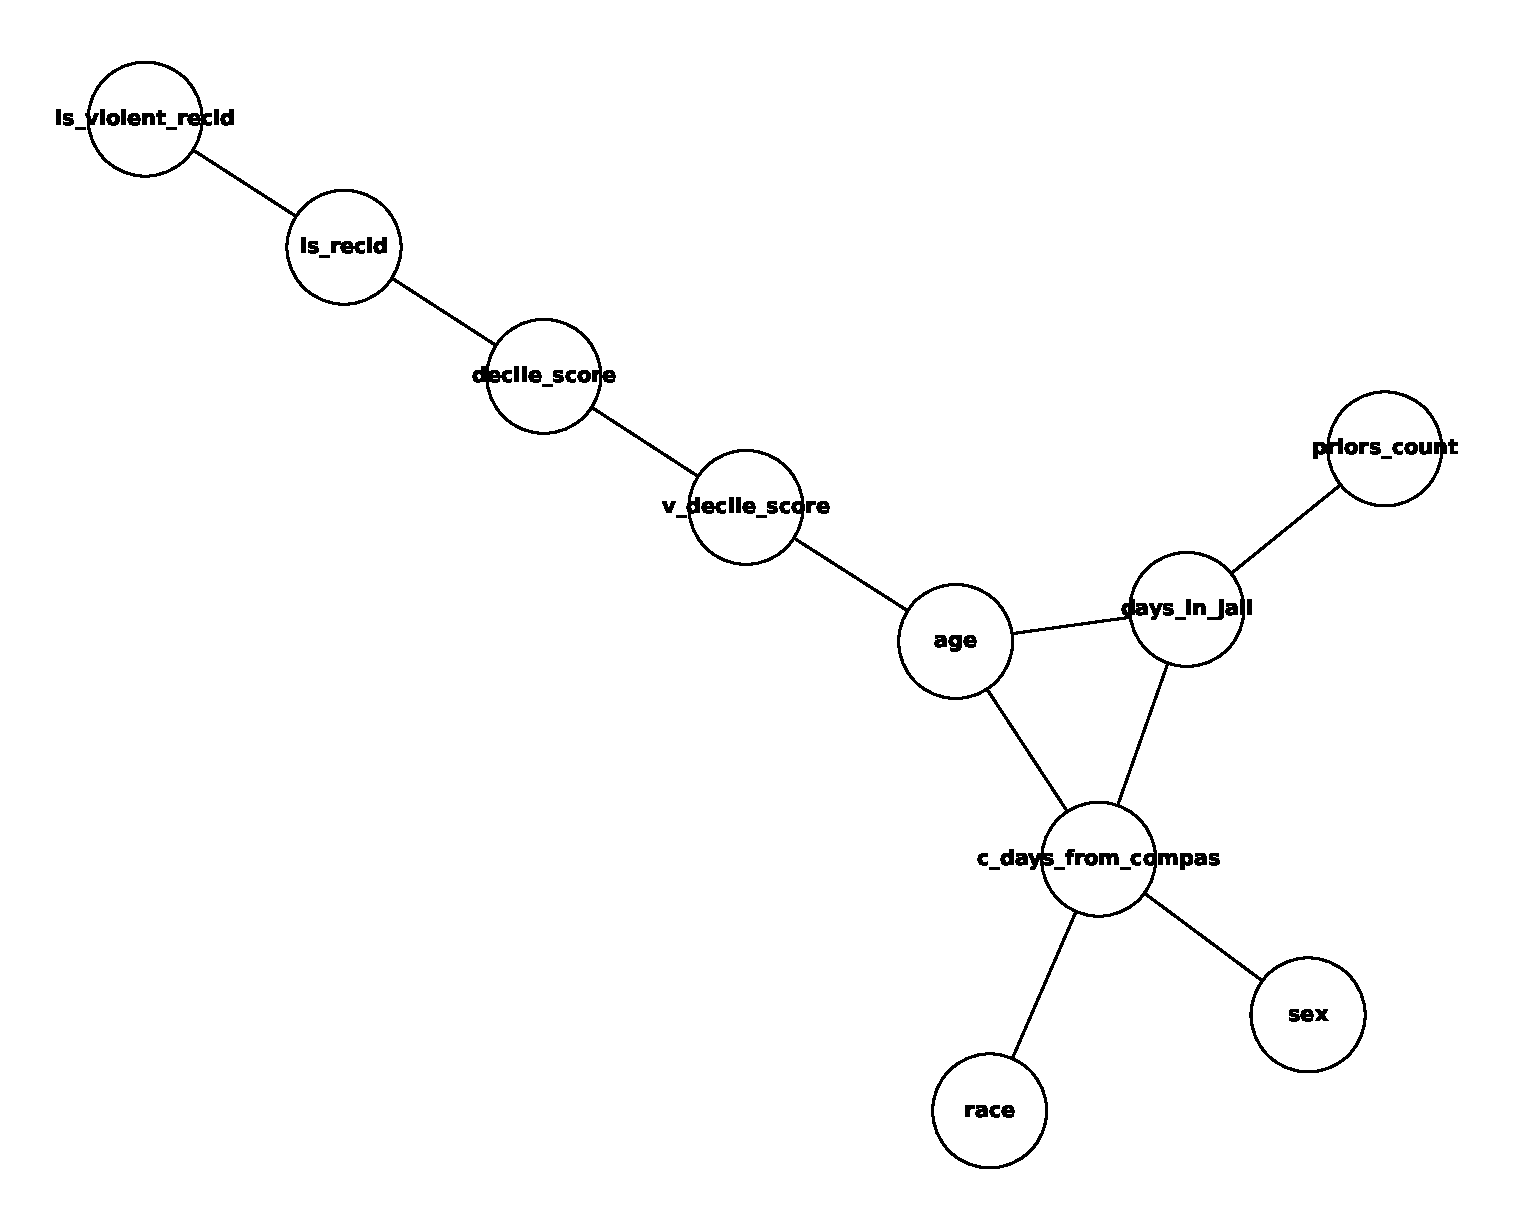
\includegraphics[width=\linewidth]{compas_mst}
%   \caption{Markov random field for marginals of the COMPAS dataset.}
%   \label{fig:compas_mst}
%   \Description{Markov random field for marginals of the COMPAS dataset.}
% \end{figure}

% \begin{figure}[h]
%   \centering
%   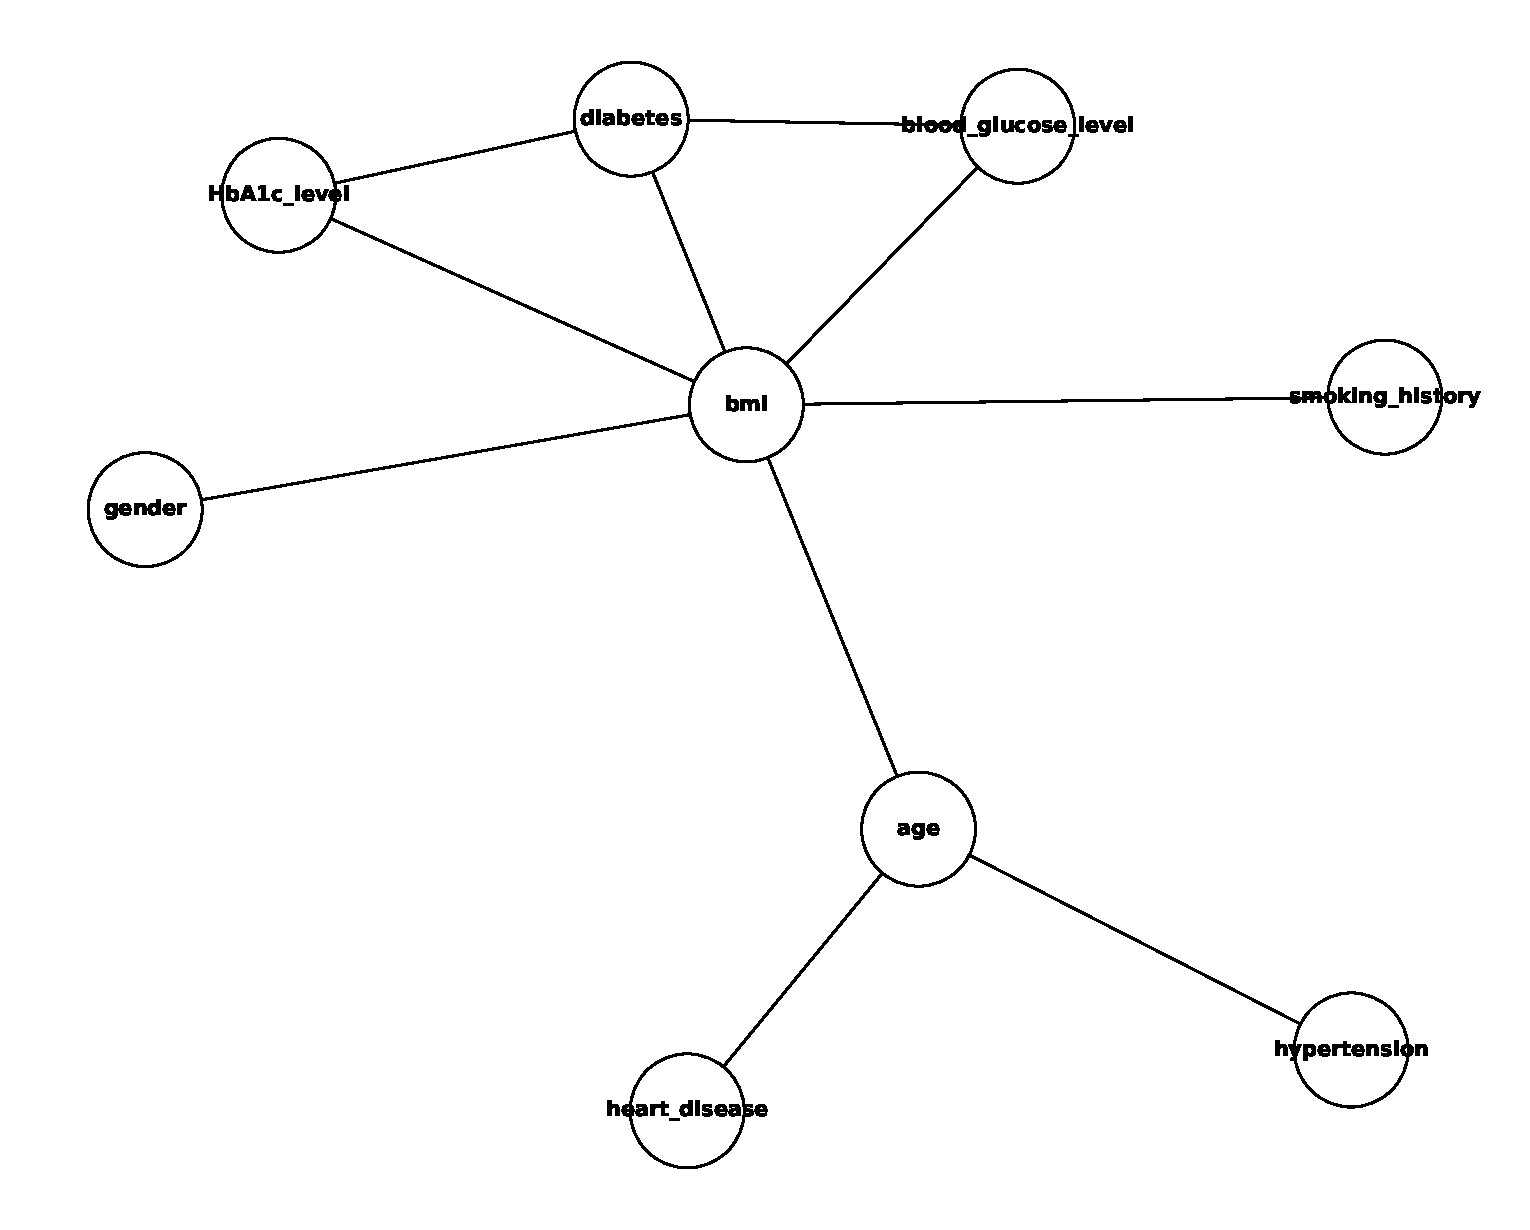
\includegraphics[width=\linewidth]{diabetes_mst}
%   \caption{Markov random field for marginals of the diabetes dataset.}
%   \label{fig:diabetes_mst}
%   \Description{Markov random field for marginals of the COMPAS dataset.}
% \end{figure}

% \begin{figure}
%   \centering
%   \begin{subfigure}[b]{0.3\textwidth}
%       \centering
%       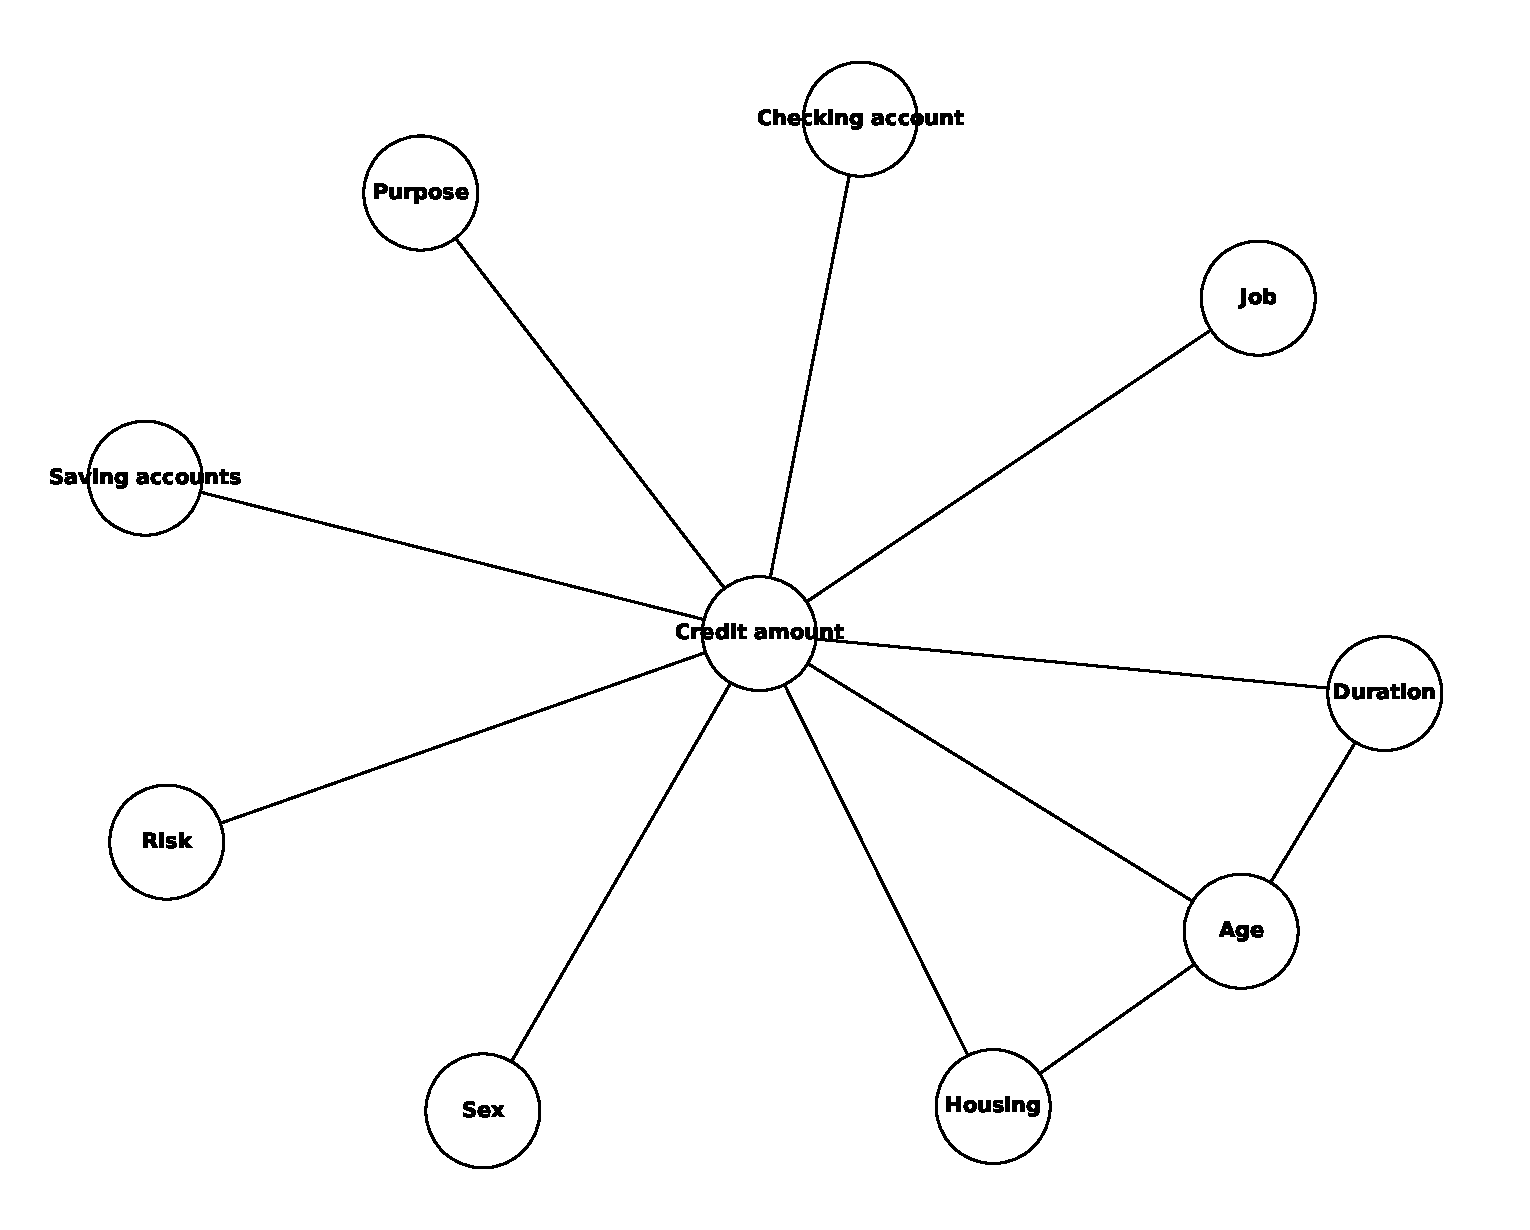
\includegraphics[width=\textwidth]{adult_mst}
%       \caption{Markov random field for marginals of the Adult dataset.}
%       \label{fig:adult_mst}
%       \Description{Markov random field for marginals of the Adult dataset.}
%   \end{subfigure}
%   \hfill
%   \begin{subfigure}[b]{0.3\textwidth}
%       \centering
%       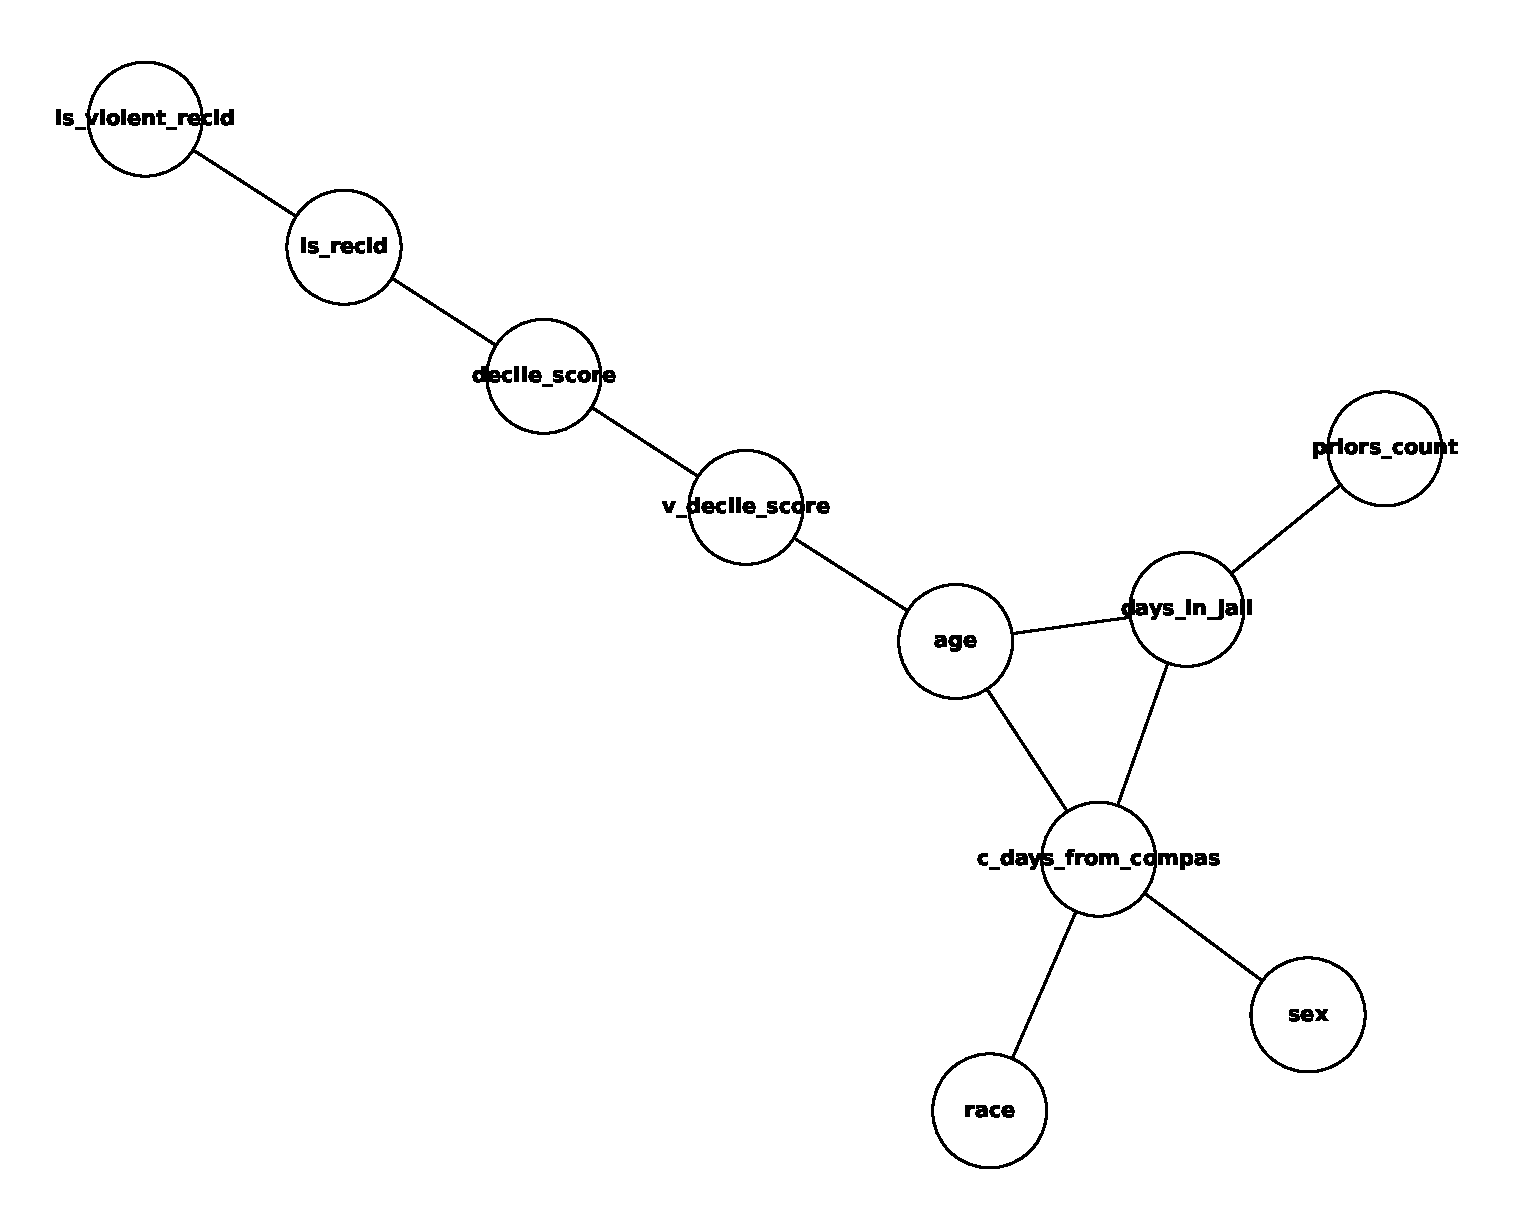
\includegraphics[width=\textwidth]{compas_mst}
%       \caption{Markov random field for marginals of the COMPAS dataset.}
%       \label{fig:compas_mst}
%       \Description{Markov random field for marginals of the COMPAS dataset.}
%   \end{subfigure}
%   \hfill
%   \begin{subfigure}[b]{0.3\textwidth}
%       \centering
%       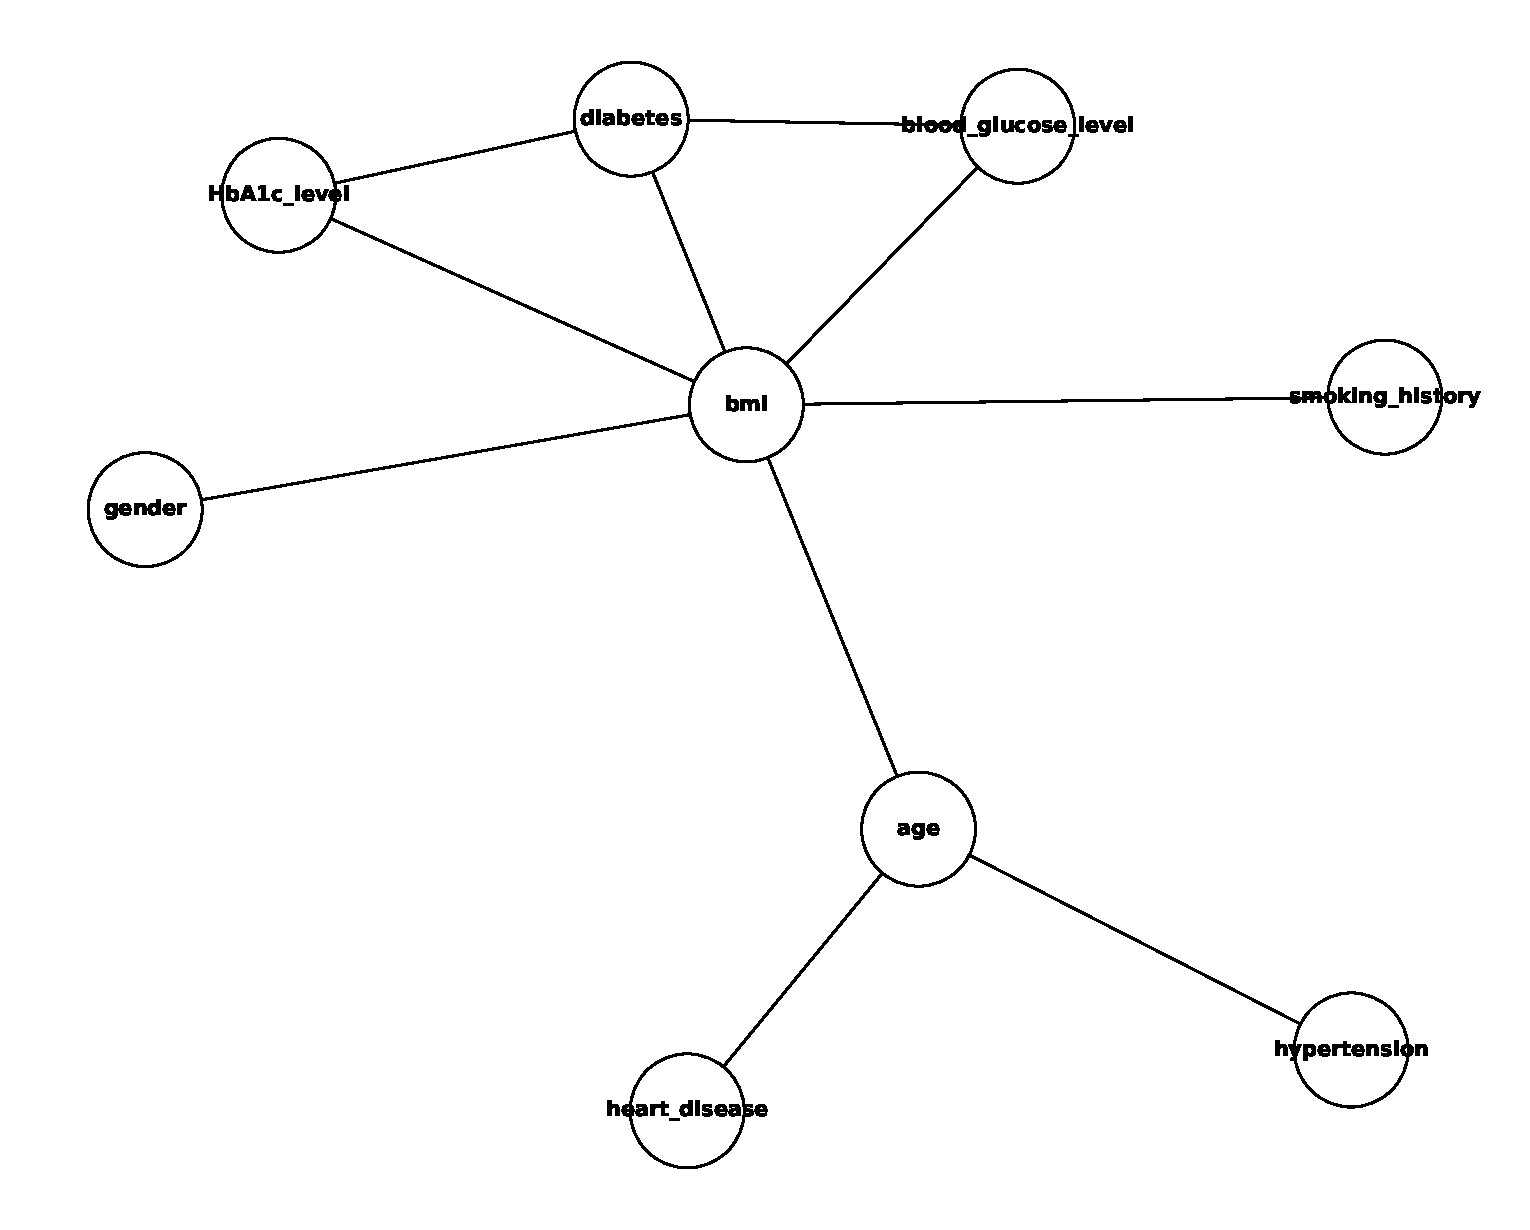
\includegraphics[width=\textwidth]{diabetes_mst}
%       \caption{Markov random field for marginals of the Diabetes dataset.}
%       \label{fig:diabetes_mst}
%       \Description{Markov random field for marginals of the COMPAS dataset.}
%   \end{subfigure}
%       \caption{Markov random field for marginals of the experimented datasets.}
%       \label{fig:msts}
% \end{figure}

\subsection{Adult Income Dataset}

The Adult\cite{adult_2,Kaggle_Adult_Census_Income} dataset comes from the 1994 census in the United States and contains about 30000 individuals. The dataset has 14 attributes, such as sex, age, and education. The task is to predict whether an individual earns more than \$50,000 a year. We set the sensitive attribute as sex and the protected group as female. The results are shown in Table~\ref{tab:adult_score}.

% For the Adult income dataset, the shape of the maximum spanning tree is very shallow, almost resembling a star; it has one internal node and all but one of the leaves have a depth of one. After introducing edges according to our heuristic, we observed an increase in the pairwise edges of the leaves, forming many 3-cliques and two 4-cliques. The resulting graph is shown in Figure~\ref{fig:adult_mst}.

% We observed that across all examined fairness measures, their difference all fall below 0.1. The average of their differences is 0.0431, which we consider quite satisfactory.

\begin{table}[h]
\caption{
    Fairness measures experiment results of the Adult dataset.
    % With heuristic, average difference is $0.0787$, and fit time is 924m15s.
    Average difference is $0.0775$, and fit time is 17m1s.
}
% \label{tab:adult_score}
% \begin{tabular}{ccccccc}
% \toprule
% \textbf{Measure} & \textbf{Original} & \textbf{Synthetic} & \textbf{difference} & \textbf{Synthetic(No Heuristic)} & \textbf{difference(No Heuristic)} \\
% \midrule
% Demographic Parity  & 0.1933 & 0.1079 & 0.0853 & 0.0114 & 0.1818 \\
% Overall Accuracy Eqaulity   & 0.0250 & 0.1399 & 0.1149 & 0.0169 & 0.0080 \\
% Equalized Odds (False Positive)    & 0.0175 & 0.0870 & 0.0695 & 0.0060 & 0.0115 \\
% Equalized Odds (True Positive)    & 0.0114 & 0.0622 & 0.0508 & 0.0303 & 0.0189 \\
% CU Accuracy Equality (True Positive) & 0.1941 & 0.1466 & 0.0474 & 0.0315 & 0.1626 \\
% CU Accuracy Equality (True Negative) & 0.1102 & 0.1450 & 0.0348 & 0.0299 & 0.0803 \\
% \bottomrule
% \end{tabular}
% \end{table}

\label{tab:adult_score}
\begin{tabular}{llll}
\toprule
\textbf{Measure} & \textbf{Original} & \textbf{Synthetic} & \textbf{Difference} \\
\midrule
Demographic Parity  & 0.1933 & 0.0114 & 0.1818 \\
Overall Accuracy Eqaulity   & 0.0250 & 0.0169 & 0.0080 \\
Equalized Odds (False Positive)    & 0.0175 & 0.0060 & 0.0115 \\
Equalized Odds (True Positive)    & 0.0114 & 0.0303 & 0.0189 \\
Conditional Use Accuracy Equality (True Positive) & 0.1941 & 0.0315 & 0.1626 \\
Conditional Use Accuracy Equality (True Negative) & 0.1102 & 0.0299 & 0.0803 \\
\bottomrule
\end{tabular}
\end{table}

\subsection{COMPAS Dataset}

The COMPAS\cite{larson2016propublica,Kaggle_COMPAS_Dataset} dataset comes from an investigative report by ProPublica of the COMPAS criminal recidivism assessment system and contains about 7000 individuals. The dataset has 10 applicable attributes, such sex, age, and priors count. The task is to predict whether an individual will re-offend. We set the sensitive attribute as sex and the protected group as female. The results are shown in Table~\ref{tab:compas_score}.

% For the COMPAS dataset, the initial spanning tree has a long tail, which is not surprising because, upon closer inspection, they all are related to the original COMPAS risk scores. The heuristic edge addition did not change the graph significantly. It only introduced one 3-clique triangle. The resulting graph is shown in Figure~\ref{fig:compas_mst}.

% The results showed an increase in error on the sufficiency measure values. In particular, one of the measures has an error difference as high as 0.141. The average of their differences is 0.069, which is worse than the adult dataset.

\begin{table}[h]
\caption{
    Fairness measures experiment results of the COMPAS dataset.
    % With heuristic, average difference is $0.0750$, and fit time is 27m33s.
    Average difference is $0.0727$, and fit time is 33s.
}
\label{tab:compas_score}
\begin{tabular}{llll}
\toprule
\textbf{Measure} & \textbf{Original} & \textbf{Synthetic} & \textbf{Difference} \\
\midrule
Demographic Parity  & 0.1310 & 0.0809 & 0.0501 \\
Overall Accuracy Eqaulity   & 0.0079 & 0.0146 & 0.0067 \\
Equalized Odds (False Positive)    & 0.0249 & 0.0802 & 0.0553 \\
Equalized Odds (True Positive)    & 0.0177 & 0.0825 & 0.0648 \\
Conditional Use Accuracy Equality (True Positive) & 0.1709 & 0.0551 & 0.1157 \\
Conditional Use Accuracy Equality (True Negative) & 0.1695 & 0.0256 & 0.1439 \\
\bottomrule
\end{tabular}
\end{table}

\subsection{Diabetes Dataset}

The Diabetes\cite{diabetes_34,Kaggle_Diabetes_Prediction} dataset comes from the hospital readmission data published in the 1994 AI in Medicine journal and contains about 100000 individuals. The dataset has 8 attributes, such as gender, age, and smoking history. The task is to predict whether an individual will be readmitted. We set the sensitive attribute as gender and the protected group as female. The results are shown in Table~\ref{tab:diabetes_score}.

% The tree grown from the diabetes dataset did not appear to have any particular characteristics. The root of the tree is placed in the BMI value, which reasonably captures most information. The heuristic edge addition process introduced some 3-clique triangles. The resulting graph is shown in Figure~\ref{fig:diabetes_mst}.

% The results showed that the synthetic data generally preserves the fairness properties of the original data.

% The average of the differences between the fairness measure values of the original and synthetic datasets is below 0.1 for all datasets. The average of the differences is 0.0431 for the adult dataset, 0.069 for the COMPAS dataset, and 0.031 for the diabetes dataset.

\begin{table}[h]
\caption{
    Fairness measures experiment results of the Diabetes dataset.
    % With heuristic, average difference is $0.0067$, and fit time is 1m44s.
    Average difference is $0.0078$, and fit time is 1m24s.
}
\label{tab:diabetes_score}
\begin{tabular}{llll}
\toprule
\textbf{Measure} & \textbf{Original} & \textbf{Synthetic} & \textbf{Difference} \\
\midrule
Demographic Parity  & 0.0135 & 0.0015 & 0.0119 \\
Overall Accuracy Eqaulity   & 0.0077 & 0.0011 & 0.0065 \\
Equalized Odds (False Positive)    & 0.0000 & 0.0010 & 0.0010 \\
Equalized Odds (True Positive)    & 0.0086 & 0.0094 & 0.0008 \\
Condtional Use Accuracy Equality (True Positive) & 0.0133 & 0.0059 & 0.0074 \\
Condtional Use Accuracy Equality (True Negative) & 0.0216 & 0.0019 & 0.0197 \\
\bottomrule
\end{tabular}
\end{table}

\section{Evaluation}

% % TODO:
% first list formulas

% count vars

% theyre not part of marginals

% they cant be computed

% we can say less about fairness with these with less info

% auditor need to know theyre aproxing scores

% auditor need to keep in mind that these scores are for datasets and we preserve these scores thats it. scores may not be accurate. it doesnt mean its less easy to test fairness

\subsection{Positive Results}

% % TODO:
% it works!

% Our experiments showed that synthetic data generally preserves the fairness properties with a reasonable degree of accuracy. The average of the differences between the fairness measure values of the original and synthetic datasets is below 0.1 for all datasets. This indicates that synthetic data is a good approximation of the original data in terms of fairness.

% For the adult dataset, the average difference was 0.0431, suggesting a close match between the synthetic and the original data in terms of fairness measures. For the diabetes dataset, the average difference was 0.031, which is even lower. Even in the case of the COMPAS dataset, which had a higher value, it was still within an acceptable range at 0.069.

% In particular, both the independence and separation measures showed low errors across all datasets, with the differences of all of them below 0.1. On the other hand, results of accuracy equality also showed low errors, with the differences of one of them as low as 0.005.

% This demonstrated that synthetic data can accurately reflect the fairness properties of the original data. Therefore, fairness analyses performed on synthetic data will yield results consistent with those on the original data.

\subsection{Negative Results}

% The experiments also revealed some limitations of this approach. In particular, the sufficiency measure showed higher errors compared to other measures. For example, in the COMPAS dataset, the sufficiency measure had an error difference as high as 0.141, while other measures had errors below 0.1.

% By close examination of our scenario, we can observe the following: of the three variables, $(\hat{Y},Y,S)$, two of them, namely $(Y,S)$, are both readily available in the original data. In contrast, $\hat{Y}$ is only available in the output of the given AI model, which cannot be captured by the synthetic data at the time of generation.

% Referring back to the definition of the fairness measures, we can see the following: separation is concerned with the form $P[\hat{Y} | S, Y] = \frac{P[\hat{Y} \cap S \cap Y]}{P[{S} \cap Y]}$, and sufficiency is concerned with the form $P[Y | S, \hat{Y}] = \frac{P[Y \cap S \cap \hat{Y}]}{P[{S} \cap \hat{Y}]}$.

% expand all defs and count the nums of avail vars

% This explains why sufficiency measures could have higher errors compared to separation because synthetic data have less information about them. While only one variable is missing in the numerator for separation, one more variable is missing in the denominator for sufficiency.

% Therefore, it is harder to approximate sufficiency measures on synthetic data. This is a fundamental limitation of this approach, and it is important to be aware of this when interpreting the results of fairness analyses.

% TODO: use = 1

\definecolor{lightgreen}{rgb}{0.6, 1.0, 0.6}
\definecolor{lightred}{rgb}{1.0, 0.6, 0.6}
\newcommand{\mathhighlight}[2]{\colorbox{#1}{$\displaystyle #2$}}
\newcommand{\y}[1]{\mathhighlight{lightgreen}{#1}}
\newcommand{\n}[1]{\mathhighlight{lightred}{#1}}

% independence
% \[
% P[\hat{Y} | S] - P[\hat{Y} | \overline{S}]
% = \frac{P[\n{\hat{Y}} \cap \y{S}]}{P[\y{S}]} - \frac{P[\n{\hat{Y}} \cap \y{\overline{S}}]}{P[\y{\overline{S}}]}
% \]

% separation
% \[
% P[\hat{Y} | S, Y] - P[\hat{Y} | \overline{S}, Y]
% = \frac{P[\n{\hat{Y}} \cap \y{S} \cap \y{Y}]}{P[\y{S} \cap \y{Y}]} - \frac{P[\n{\hat{Y}} \cap \y{\overline{S}} \cap \y{Y}]}{P[\y{\overline{S}} \cap \y{Y}]}
% \]

% sufficiency
% \[
% P[Y | S, \hat{Y}] - P[Y | \overline{S}, \hat{Y}]
% = \frac{P[\y{Y} \cap \y{S} \cap \n{\hat{Y}}]}{P[\y{S} \cap \n{\hat{Y}}]} - \frac{P[\y{Y} \cap \y{\overline{S}} \cap \n{\hat{Y}}]}{P[\y{\overline{S}} \cap \n{\hat{Y}}]}
% \]

% accuracy equality
% \[
% P[Y = \hat{Y} | {S} ] - P[Y = \hat{Y} | \overline{S}]
% = \frac{P[\y{Y} = \n{\hat{Y}} \cap \y{S}]}{P[\y{S}]} - \frac{P[\y{Y} = \n{\hat{Y}} \cap \y{\overline{S}}]}{P[\y{\overline{S}}]}
% \]

\section{Conclusion}


%%
%% The acknowledgments section is defined using the "acks" environment
%% (and NOT an unnumbered section). This ensures the proper
%% identification of the section in the article metadata, and the
%% consistent spelling of the heading.
% \begin{acks}
% To Robert, for the bagels and explaining CMYK and color spaces.
% \end{acks}

%%
%% The next two lines define the bibliography style to be used, and
%% the bibliography file.
\bibliographystyle{ACM-Reference-Format}
\bibliography{references}


%%
%% If your work has an appendix, this is the place to put it.
% \appendix

\end{document}
\endinput
%%
%% End of file `sample-manuscript.tex'.
